\chapter{Proposal of parallel approach}
\label{04:chapter:title}

In this chapter, the author describes the overall design for parallelism the computation of the Strimzi system tests.
At first, Section~\ref{05:bottlenecks} explains the prevailing problems in the Strimzi system tests.
Then, Section~\ref{05:possibleapproaches} describes alternatives to solve these problems.
Finally, the best possible option is proposed that meets all the necessary needs.
Next, in Section~\ref{04:architecturechanges} we propose changes that have to be made, especially in the \emph{ResourceManager}, where the current algorithms for resource management are implemented and which currently do not support a thread-safe implementation.
Finally, in Section~\ref{04:methodwideparalelisation} and Section~\ref{04:classwideparalelisation} a proposal for \emph{method-wide} and \emph{class-wide} parallelisation is specified, which is described in detail with the steps that need to be done for its construction (conflicts it contains and solutions proposed using learned knowledge from previous chapters).

\section{Bottlenecks of current approach}
\label{05:bottlenecks}

As discussed in Section~\ref{02:sec:strimzisystemtests}, the time required for a given test set is extremely time-consuming.
It is easier to maintain the correctness of a program using the sequential computing model, but the benefit that parallelism offers are hard to ignore.
Nevertheless, one has to ask oneself whether it is possible and whether it worth the investment.
To answer such a question, we can use Amdahl's law, which we learned about in Section~\ref{04:amdalhlaw}.
For simplicity, assume that the unit of work will be a test case.
It will therefore be necessary to map how many tests can be parallelised.
We can find out that by analysing whether a test case contains any shared variable with other tests (i.e., shared \emph{Kafka, KafkaMirrorMaker, KafkaConnect, KafkaUser, KafkaTopic resource}).
Once it does not contain any variable, we can declare the test as parallelisable.
If a given test contains such a shared variable, it implies that it will have to run in an isolated environment.
The manual analysis we performed found that 250 tests could be run in parallel, and 115 must be isolated.
So if we apply Equation~\eqref{eqn:einstein}, (which we learned in Section~\ref{04:amdalhlaw}), the total number of tests is 365.
The parallelizable part is \emph{p = 250/365}.
The sequence part will be equal to \emph{seq = 1 - p = 115/365}.
For only four-core CPUs, we get the following acceleration~\eqref{eqn:amdalhinpractice}.
\begin{equation}
    \label{eqn:amdalhinpractice}
    S = \frac{1}{1 - \frac{250}{365} + \frac{\frac{250}{365}}{\frac{4}{1}}} =\sim 2.1x \; acceleration
    \tag{3}
\end{equation}
If we increase the number of CPUs to 8, the total acceleration will be 2.5 times, and if we scale it to 16 CPUs, the acceleration will be almost 3 times.
Consequently, if we imagine that our system tests have a total executive time of 40 hours, all tests will last approximately 13 hours with parallelisation.
Thus, with this first step, we just showed that it pays to parallelise.

Another disadvantage of the current approach is that it does not use multiple Namespaces.
In our case, for each test suite, we always have one Namespace in which we operate.
Parallelism allows us to manage multiple namespaces simultaneously while ensuring that the test cases do not overlap.
Subsequently, we create in each Namespace a Cluster Operator, again and again;
this process usually takes one minute.
The ideal approach should be that the Cluster Operator should see all Namespaces and shared them for all test suites.
Using this approach eliminates much lost time.
However, we must be aware of a particular test suite or the test case that will require a different Cluster Operator configuration.
At that moment, we must guarantee that some label will annotate that single test case for the entire test suite to run in isolation.

The disadvantages of the current approach mentioned above may be a clear argument for why such a change is necessary.
What is also necessary to mention is the structure of the Resources classes in the Strimzi system tests.
These are classes that encapsulate both, a pre-prepared templates and, at the same time, the whole mechanism of creation.
\begin{figure}[!ht]
    \centering
    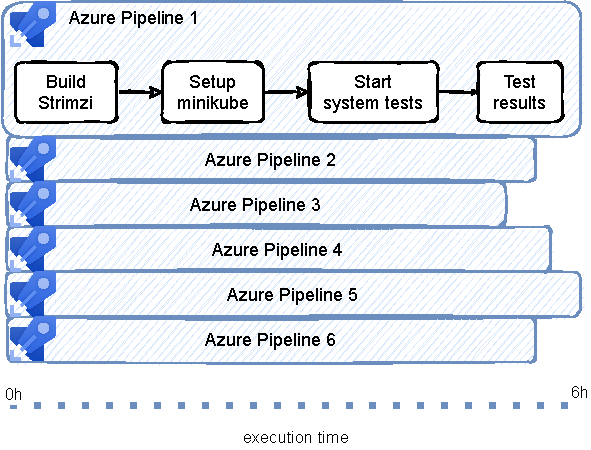
\includegraphics[scale=1]{obrazky-figures/06-proposal-of-parallel-approach/01a-azure_pipelines_with_test_results}
    \caption{Azure pipelines in form parallelism used to execute our system tests}
    \label{05:fig:azurepiplines}
\end{figure}
If we want to create a resource, we do it using \emph{KafkaResource.kafkaEphemeral(...).done()} method calls and similarly with other resources.
The correct API should propagate everything for the client writing the tests via the \emph{ResourceManager} class where a simple \emph{create()} method would be called.
Nevertheless, this fact is more a matter of architecture and not a form of the execution model.

Finally, we can discuss the last limitation for which it is necessary to make a change.
In the~\ref{02:sec:strimzisystemtests} section, we did not mention such a fact, but there is an attempt of parallelism when using the Microsoft Azure Pipelines.
On this infrastructure, we decompose our system tests into several distinctive subsets and run them as Azure separate pipelines\footnote{\textbf{Azure pipeline} \---\ one can imagine pipeline, as an Object which encapsulates multiple commands executed in order. Moreover, it is also executed as a separate process.}.
In Figure~\ref{05:fig:azurepiplines} one can see such decomposition.
The attentive reader might ask why we cannot run 40 or 100 Azure pipelines and thus reduce the total execution time of the tests.
Unfortunately, we are limited only to run six Azure Pipelines simultaneously.
By this limitation, the total set of tests takes approximately 6 hours, which is still a significant ammount of time.
Similarly, we try to reduce the time at the Jenkins pipeline when using OpenStack\footnote{\textbf{OpenStack} \---\ is a cloud computing infrastructure that manages physical machines, virtual servers or containers. At the same time, this product is one of the three most active open-sourced products globally. (\url{https://www.openstack.org/})} and Amazon Web Services infrastructure\footnote{\textbf{Amazon Web Services} \---\ also like OpenStack, is a cloud computing infrastructure that offers a myriad of services (i.e., Amazon Elastic Compute Cloud, Amazon Simple Storage Service). A very admirable attribute of this service is the availability level according to SLA (service level agreement) up to 99.9\%. (\url{https://aws.amazon.com/})}.
However, this Strimzi product must be verified for multiple configurations when running a separate Kubernetes cluster for the entire test suite.
Once we launch several such Kubernetes clusters, we are also limited by infrastructure quotas.
Overall execution time reduced can be seen in the following Figure~\ref{05:fig:jenkinspipelines}.
\begin{figure}[!ht]
    \centering
    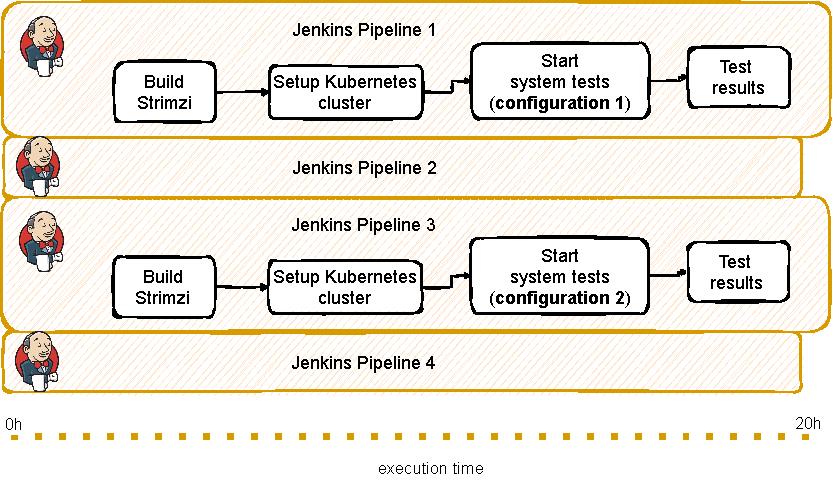
\includegraphics[scale=1]{obrazky-figures/06-proposal-of-parallel-approach/02-jenkins-smaller}
    \caption{Jenkins pipelines in a form parallelism used to execute our system tests}
    \label{05:fig:jenkinspipelines}
\end{figure}

It is also important to mention that we are limited by the number of processes (i.e., pipelines) that always use the separate Kubernetes cluster.
On Amazon Web Services and Openstack infrastructures, we are not limited the computing resources we use.
This is the fact that we must use and thus think about how parallelisation will lead the way.
Undoubtedly, this will not be at the levels of processes, but parallelisation is possible directly in the test set (i.e., using threads) thanks to the available computational resources.
However, this decision evokes the approaches described in the next section.

\section{Possible approaches}
\label{05:possibleapproaches}

From the previous section, we could notice that any attempt to parallelise at the process level (i.e., spawn more pipelines) was impossible, especially in terms of individual infrastructures' constraints.
As a result, we have no choice but to go one level lower and try to parallelise at the test level and thus use the threads.

\subsection{Writing own testing framework}

The first and the most difficult alternative is to write a new testing framework.
One would say that this may be an old-fashion approach, but it also has its advantages.
One of the leading benefits is flexibility.
Imagine that we want to configure how many test cases and test suites we want to run simultaneously.
The natural way to do this is using Futures.
Each parallel suit is associated with its \emph{Future}, and one uses a composite future to await the completion of all of them.
We could do that by using \emph{JDK ExecutorService}\footnote{\textbf{ExecutorService} \---\ is a Java object, which provides a way to execute tasks on threads asynchronously.} and \emph{CompletableFuture}\footnote{\textbf{CompletableFuture} \---\ is a superset to Future, which we learned about at the end of Chapter \ref{03:chapter:title}. Moreover, it provides exception handling, allows us to combine CompletableFuture, and has many auxiliary methods}.
However, the problem that writing a new tool would mean writing new tests and partially rewriting them all.
Since our tests are currently designed on top of the JUnit5 platform, it is not very acceptable for us to do such a thing.

\subsection{Writing our own Junit5 Engine}

Another alternative to reduce the overall load of rewriting all tests would be to write a new JUnit5 Engine.
In this case, we would have to write the overall logic of the lifecycle test.
It would help if one remembered how we described the dependencies of the current Strimzi system tests in Section~\ref{02:subsec:strimziJunit5relation:execution}.
This dependency eliminates the worry of \emph{TestDiscovery} and \emph{TestExecution}.
Therefore, if we want to create our own \emph{TestEngine}, we have to implement our own \emph{TestDiscovery} and thus create our own implementation similar to Algorithm~\ref{02:alg:selectorresolver}.
Furthermore, we need to create our own \emph{TestExecution} mechanism.
The testing mechanism could be very similar to the previous subsection, thus using the \emph{CompletableFutures} and \emph{ExecutorService} classes that Java offers.
One may invoke the idea that this is the best approach that eliminates the discovery of all tests and the overall work on designing a new tool.
Unfortunately, it also has its disadvantages.
One of them is that if one decides to write their \emph{TestEngine}, they must realise that this eliminates all the annotation support offered by Junit5 \emph{TestEngine} (i.e., @Test, @TestFactory, @ParametrizedTest, @Isolated and @TestTemplate).
It is clear that if we write a new \emph{TestEngine}, we have to write our own annotated tests and write our own annotations.
With this knowledge, even this approach does not meet our needs.


\subsection{JUnit5 paralelization}

The last alternative is the use of Junit5 \emph{TestEngine} parallelisation.
This, almost 3-year-old, feature of the Junit5 platform (released 3rd September in 2018) has a lot to offer.
For example, parallelisation support for running multiple test cases at one time is possible using the \emph{Java Fork / Join} framework.
This framework also includes the implementation of the \emph{ThreadPool} object, which we described in Chapter \ref{03:chapter:title}.
The overall logic utilises reusable Threads, where, for example.
Thread A completes the execution of Test 1, it will be assigned another test immediately and thus, we eliminate redundant creation of threads.
The main advantage of such an approach is that it is not necessary to rewrite a complete perform of the tests.
Moreover, it is unnecessary to implement TestDiscovery and TestExecution because JUnit5 TestEngine already offers them.
Related to this is keeping all the annotations mentioned in the previous subsection.
Another advantage is the possibility of configuration where we can enable parallelization using the following commands:
\begin{verbatim}
junit.jupiter.execution.parallel.enabled = true
junit.jupiter.execution.parallel.mode.default = same_thread
junit.jupiter.execution.parallel.mode.classes.default = concurrent
\end{verbatim}
With this setting, it is possible to run the suite test in parallel using Junit5 parallelisation.
If we change \emph{junit.jupiter.execution.parallel.mode.default = concurrent} then we let concurrent execution of test cases and test suite run simultaneously.
Another good aspect of this feature is the ability to choose the best variant of the parallelisation strategy:
\begin{itemize}[itemsep=1mm, parsep=0pt]
    \item \textbf{Fixed} \---\ \emph{ThreadPool} has a predefined number of threads to work with and can be changed in the configuration using \emph{parallel.config.fixed.parallelism}.
    \item \textbf{Dynamic} \---\ \emph{ThreadPool} has a predefined number of threads based on the calculated available processors multiplied by the number specified by \emph{parallel.config.dynamic.factor}.
    \item \textbf{Custom} \---\ possible custom implementation of the strategy.
\end{itemize}
However, this configuration does not apply to scenarios where we want to run a particular set of tests in parallel and the other sequentially.
Therefore, Junit5 also provides a possible dynamic rewrite of the configuration at build time using the @Execution annotation, which can contain two values for sequential execution (@Execution (SAME\_THREAD) ) of a test suite or test case or @Execution (CONCURRENT) for concurrent execution of class or test case.
Thanks to the mentioned annotations, we can achieve decompositions of tests that will run in parallel and sequentially.
It may be apparent to the reader that our needs will be met by using this feature of the Junit5 Engine offers.

However, another common problem with the approach we have described is that the current ResourceManagement is not ready for parallelisation.
This problem forces us to rewrite our test architecture, and with that comes the rewriting of the ResourceManager class and its Resource classes.

\section{Architecture changes}
\label{04:architecturechanges}

In this section, we will describe all the necessary changes in our system test architecture.
We start with designing thread-safe algorithms responsible for managing the resources with which the individual test cases operate.
Finally, we describe the design of individual resource classes that will use the Interface pattern\footnote{\textbf{Interface pattern} \---\ one of the most popular design patterns, which defines a set of operations and creates a contract for a class that must implement these operations.}

\subsection{Resource classes}

If we think about the whole architecture of the system tests from the section~\ref{02:sec:strimzisystemtests}, one will notice that the Resource classes contains two large pieces.
The first are management methods (i.e., create(), delete()), and the second part are predefined templates, which are then used in test cases.
Therefore, we suggest that the given parts of the code must be divided into classes, where the methods are used for management would be left in these classes.
However, predefined templates moved to the so-called \emph{Templates} classes.
With further improvements and better design, we propose to create an interface that will contain methods for resource management, and each type of Resource class will need to implement such an interface.
The given interface should consist of the following abstract methods:
\begin{itemize}[itemsep = 1mm, parsep = 0pt]
    \item \textbf {getKind()} \---\ an abstract method that will serve as a type identifier of the given resource instance,
    \item \textbf {get()} \---\ the abstract method that will serve as a single resource,
    \item \textbf {create()} \---\ the abstract method responsible for creating the resource,
    \item \textbf {delete()} \---\ the abstract method responsible for deleting a given resource,
    \item \textbf {waitForReadiness()} \---\ the abstract method, for waiting for a given resource until it is ready.
\end{itemize}
Thanks to this change, we will create a generic method at the heart of the ResourceManager class.

\subsection{ResourceManager}

The most critical part of system test module is ResourceManager.
In Section~\ref{02:sec:strimzisystemtests}, we described how this class works and what exactly it contains.
To maintain the context of all resources with which the three types of stacks are currently used.
If we are in the \emph{@BeforeAll} context, then it is clear that we switch the pointer stack to the class stack.
On the other hand, before each test case, we switch to the method stack.
However, the cautious reader will realise that such a mechanism will not work in parallel executions.

As part of the change, we propose eliminating all three stacks used to maintain the context and creating a HashMap that will have the name of the test case as an identifier (key).
We create a contract for a person who creates the tests to do not equal themselves.
As a value in the given map, we will store a Stack that will store all types of resources, i.e. there will always be one stack for each test case.
Related to this section is a change in resource creation management.
We propose the following thread-safe algorithm~\ref{04:alg:creationofresource}, which eliminates the invocation of methods from individual Resource classes, but all this will be done within the ResourceManager class.
In the given algorithm, there are 3 phases:

\begin{itemize}[itemsep=1mm, parsep=0pt]
    \item \textbf{Find} \---\ finding the resource type and invoking it within the Kubernetes API,
    \item \textbf {Store and future deletion} \---\ save the resource to the stack and automatically delete it throughout the lifecycle,
    \item \textbf {Readiness check} \---\ waiting if a given resource is deployed in a Kubernetes cluster (optional).
\end{itemize}

\begin{algorithm}[H]
    \label{04:alg:creationofresource}
    \caption{Thread-safe algorithm for creation resources inside \emph{Resource manager}}

    \hspace*{\algorithmicindent} \textbf{Input: ExtensionContext context, GenericType resources}

    \begin{algorithmic}[1]
        \ForEach{$resource \in resources$}
        \State $type \gets findResourceType(resource)$
        \State $type.create(resource)$
        \State // here starts critical section
        \State $all\_resources.computeIfAbsent((test\_name), k -> new Stack<>())$
        \State $all\_resources.get((test\_name).push(deleteResource(resource)$
        \State // here ends critical section
        \If{wait for resource readiness}
            \ForEach{$resource \in resources$}
            \State $type \gets findResourceType(resource)$
            \State wait for resource readiness
            \EndForEach
        \EndIf
        \EndForEach
    \end{algorithmic}
\end{algorithm}

An essential aspect of this proposed algorithm is also the ExtensionContext, which will identify the current place of execution.
There is an ExtensionContext for each test case and it contains metadata about the test.

Another part is in case the user wants to asynchronously create ten resource instances independently of each other and then create a Barrier\footnote {\textbf{Barrier} \---\ is a mechanism in concurrency, which is used to synchronise multiple threads\/processes. Therefore, any thread\/process has to wait for all the threads\/processes in that place. Subsequently, if all threads\/processes arrive at the given place, the threads\/processes are awakened and can continue their execution} because the following verification steps require all resources.
Another thread-safe algorithm~\ref{04:alg:syncresources} does a very similar process, waiting for all resources to be created asynchronously.
The identification of which resource to wait for is within the given ExtensionContext.

\begin{algorithm}[H]
    \label{04:alg:syncresources}
    \caption{Thread-safe algorithm for sychronising resources inside the \emph{Resource manager}}
    \hspace*{\algorithmicindent} \textbf{Input: ExtensionContext context}
    \begin{algorithmic}[1]
        \State Stack<Resource> resources = resourceStack.get(context.getTestName());
        \State

        \State // sync all resources
        \ForEach{$resource \in resources$}
        \If{$resource == null$}
            \State $continue;$
        \EndIf

        \State
        \State {$type \gets findResourceType(resource)$}

        \State {$\Phi \gets getResourceWaitCondition(type)$}
        \State {$wait(resource, \Phi)$}
        \EndForEach
    \end{algorithmic}
\end{algorithm}

Finally, we have the last part, that is deleting resources from the stacks.
We propose a thread-safe algorithm~\ref{04:alg:deleteresources}, which will be used for the overall cleaning of the test environment.
Its functionality is configurable.
In the beginning, it finds out the condition of the emptiness of the map that contains all the resources.
Subsequently, if it does not contain anything, the whole execution ends.
However, if the map is not empty, deletion begins.
Once this phase is completed, everything will be deleted from the map.

\begin{algorithm}[H]
    \label{04:alg:deleteresources}
    \caption{Thread-safe algorithm for deletion of resources the inside \emph{Resource manager}}
    \hspace*{\algorithmicindent} \textbf{Input: ExtensionContext context}
    \begin{algorithmic}[1]
        \State{$\Psi \gets mapResourceEmptinessCondition(context)$}

        \If{$\Psi$}
            \State{$break;$ // everything is deleted}
        \EndIf
        \While {$!\Psi$}
            \State{// checking if some exception in scope of extension context arised}
            \State{$resources.get(context.getDisplayName()).pop().getThrowableRunner().run();$}
        \EndWhile

        \State{// remove stack from map}
        \State{$resources.remove(context.getDisplayName());$}
    \end{algorithmic}
\end{algorithm}

\section{Method wide paralelization}
\label{04:methodwideparalelisation}

In this section, we will describe our proposal for a possible method-wide parallelisation.
Method-wide parallelisation is where each test suite will be isolated, and each test case will run in parallel, if possible.
We have already approached the condition for running the tests in parallel in Section~\ref{05:bottlenecks}.
So this is a test that does not use any shared resources.
The proposal is decomposed into several steps: which are described in the next paragraphs.

The first step is to create a unique name mechanism for all the resources that are used in the test cases.
Since these are Kubernetes system tests, the created resources do not have a random naming generated.
By randomisation, we eliminate possible conflicts that could arise in parallel execution in a given test suite.
Furthermore, random naming does not require additional synchronisation of conflicting resources because each newly created resource will have a different name.

The second step is to create Kubernetes methods that will support namespace operations.
Thanks to the Kubernetes client, which we already have in the system tests, this is possible.
However, it contains too complicated invocations of methods, and so for our purposes, it is better to encapsulate this complexity into factory methods.
These are mainly methods for communication with the Kubernetes environment (i.e., Pod, ReplicaSet, Deployment, Services, Custom Resource, Custom Resource Definition).

The third step provides a mechanism that determines which methods can be performed in parallel and which need to be isolated.
For parallel tests, we propose use the \emph{@ParallelTest} annotation.
This annotation will encapsulate the \emph{@Test} annotation, so the JUnit5 framework recognises it as a test.
It will also be necessary to add information so that the test can run in parallel.
\begin{figure}[!ht]
    \centering
    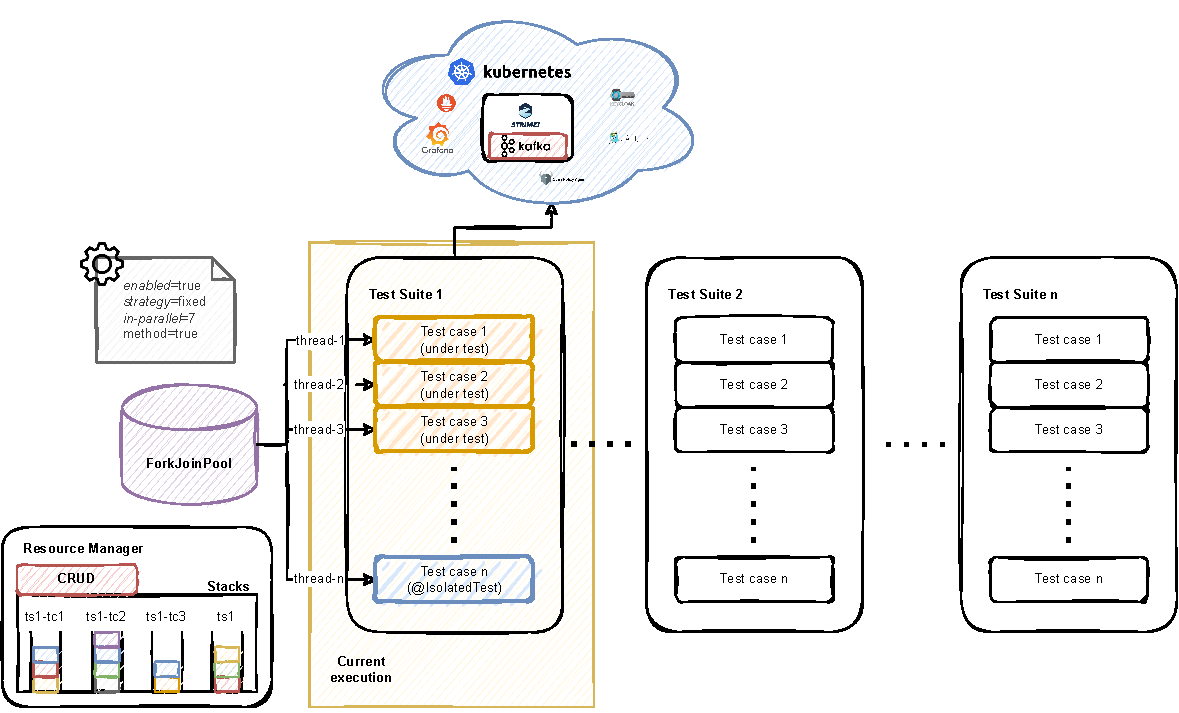
\includegraphics[scale=0.8]{obrazky-figures/06-proposal-of-parallel-approach/04-method-wide}
    \caption{The best scenario in \emph{method-wide} parallelism. \emph{n} number of threads are executed, and there is no one \emph{@IsolatedTest} in the test suite, which means that all test runs simultaneously. Note that \emph{Tc} means Test case in short.}
    \label{05:fig:methodwideparallelism}
\end{figure}
Thanks to the @Execution annotation, which will be set to the value \emph{CONCURRENT}, the test will always run in parallel.
On the other hand, tests that will require isolation will use @IsolatedTest annotation.
This annotation will be a bit more complex because it will contain not only the @Test annotation but also the read-write lock.
As a reminder from Chapter~\ref{03:chapter:title}, read-write lock consists of two types of locks.
ReaderLock allows multiple readers to read from a shared source.
However, if even one reader reads, no thread can write to the source.
If no reader reads anymore and one thread wants to write, the file will be locked using WriterLock.
Here, however, another thread cannot access until the same thread rereleases it.
So for the @IsolatedTest annotation, we propose using this type of lock to guarantee the system's safety property (mutual exclusion).

In Figure~\ref {05:fig:methodwideparallelism} it is possible to see the best scenario that can happen in \emph {method-wide} parallelisation.
Moreover, we must realise that if the test suite theoretically contains all \emph{@IsolatedTest}, it would be a sequential execution.
Of course, if the computer on which the tests would run contained no more than two CPUs, then it is not possible to run multiple parallel threads with each other (it is possible, but the processor would then have to make many \textbf{context switches}, which would lead to a significant decrease in performance).
Thus, the more CPUs a given computer/cluster will have available, the quickier the results.

\section{Class wide paralelization}
\label{04:classwideparalelisation}

In this section, we will describe and suggest what steps are needed to support \emph{class-wide} parallelisation.
At first, in Section \ref{05:sharedclusteroperator}, we describe all the necessary changes that need to be made.
Furthermore, restructuring and creating a new class for managing all possible Cluster Operator configurations.
Next, we describe the rollback mechanism needed to solve the problem with two test suites that need different configurations.
Finally, we follow up on this in Section \ref{05:isolatedsuite}, where we solve the given problem completely.

\subsection{Shared Cluster Operator}
\label{05:sharedclusteroperator}

This change requires multiple interventions in the test suite.
Since a new Cluster Operator is currently being created in each test suite, we must always have this Cluster Operator available in a shared context.
This is accompanied by the question of how it will be possible to obtain such a context.
In Section \ref{04:architecturechanges}, especially in the description of the ResourceManager component, we partially described the ExtensionContext object, which serves as a test identifier thanks to a \emph{hashcode}\footnote{\textbf{Hashcode} \---\ hashcode in Java is usually an integer value that has the same number for the identical objects. However, if the objects differ in one of the instance attributes, the hashcode must have a different value. This is a known contract between a Class and its implemented \emph{int hashCode()} method.}  However, we must be aware that any ExtensionContext in either the \emph{@BeforeEach} or \emph{@BeforeAll} scopes of the code cannot be used. If we used such an ExtensionContext, the Shared Cluster Operator would be deleted after the test suite in \emph{@AfterAll} has perished. One elegant approach to solving this problem is to use the \emph{extensioncontext.getRoot()} context, which ensures that the Cluster Operator is not deleted prematurely.
Another problem is the lack of an annotation/extension that creates a shared Cluster Operator only once if multiple test suites are run.
We propose to create such an annotation \emph{@BeforeAllOnce}.
Thanks to JUnit5 and its flexibility, it will be possible to implement such a mechanism by overriding \emph{@BeforeAllCallback}.

Another significant change that needs to be made is the unification of the Cluster Operator installation.
This requires a design that encapsulates multiple configurations of the Cluster Operator and would be easy to use for the client.
The answer to this is the \emph{Builder design pattern}, which will allow the client to specify the necessary configuration it will require.
On the other hand, a person implementing this mechanism will disable parts that he does not want to make available to the user using operators' visibility (i.e., private, protected, package-protected).
This eliminates the number of factory methods currently in the project and increases the overall readability of the code.
An example of the resulting implementation and invocation for a given client might look exactly like the code shown in \ref{05:fig:clusteroperatorinstallation}.

\begin{figure}[ht!]
    \centering
    \begin{verbatim}
    // cluster operator deployment configuration
    clusterOperatorDeployment = new SetupClusterOperatorBuilder()
        (1) .withClusterOperatorName("my-cluster-operator")
        (2) .withExtensionContext(sharedExtensionContext)
        (3) .withNamespace("infrastructure-namespace")
        (4) .withWatchingNamespaces("*")
        (5) .withOperationTimeout(...)
        (6) .withReconciliationInterval(...)
        (7) .withExtraEnvVars(...)
        (8) .createInstallation()
            .runInstallation();
    \end{verbatim}
    \caption{One of the possible invocation of Cluster Operator deployment using the Builder desing pattern.}
    \label{05:fig:clusteroperatorinstallation}
\end{figure}

This may not be clear from the Figure~\ref{05:fig:clusteroperatorinstallation}, but the \emph{runInstallation()} method should encapsulate all installations such as RBAC, HELM, and BUNDLE. Each of these installations has its preparation of the environment, and therefore it is necessary to distinguish them. For clarity, we will also describe the individual parameters that we indicated in Figure~\ref{05:fig:clusteroperatorinstallation}.

\begin{enumerate}[itemsep = 1mm, parsep = 0pt]
    \item \textbf{withClusterOperatorName} \---\ will be used to specify the exact name of the Cluster Operator Deployment.
    \item \textbf{withExtensionContext} \---\ possible ExtensionContext specification for resource management.
    In this case, a shared ExtensionContext object that will ensure that the instance is not deleted prematurely.
    \item \textbf{withNamespace} \---\ specification of the Namespace name to be created for the Cluster Operator.
    In this case, the infrastructure Namespace is used.
    \item \textbf{withWatchingNamespaces} \---\ specification of the Namespaces that the Cluster Operator must observe.
    In most cases, this will be a configuration where the Cluster Operator is set to \emph{*}, which semantically means that it observes all Namespaces available in the Kubernetes cluster.
    \item \textbf{withOperationTimeout} \---\ timeout specification for Cluster Operator internal operations (ie, Kafka cluster, Kafka Mirror Maker creation).
    \item \textbf{withReconciliationInterval} \---\ specification of the control loop loop interval.
    \item \textbf{withExtraEnvVars} \---\ additional possible configurations using environment variables (i.e., Strimzi operator namespace labels or Strimzi network policy generation).
    \item \textbf{createInstallation} \---\ instance construction with pre-supplied attributes.
\end{enumerate}

The last change within the shared Cluster Operator is to create a rollback mechanism that will solve the problem if we have two test suites with different Cluster Operator configurations.
Note that it is not possible to have multiple Cluster Operator deployments, as this would overlap and at the same time disrupt the operators.
Therefore, we propose to create a rollback mechanism that will solve this problem. The~\ref{05:alg:rollback} algorithm shows the principle of operation.
Specifically, we suggest that the algorithm be divided into two phases, where the first is to delete all currently deployed resources.
The second phase is the deployment of a new Cluster Operator with a default configuration.
\begin{algorithm}[H]
    \label{05:alg:rollback}
    \caption{Cluster Operator rollback algorithm}
    \begin{algorithmic}[1]
        \State{$// \; 1st \; phase$}
        \State{// trigger that we will again create namespace}
        \If{Environment.isHelmInstall()}
            \State{helmResource.delete();}
        \EndIf
        \If{Environment.isOlmInstall()}
            \State{olmResource.delete();}
        \EndIf
        \If{Environment.isBundleInstall()}
            \State{// clear all resources related to the extension context}
            \State{ResourceManager.getInstance().deleteResources(sharedExtensionContext));}
            \State{KubeClusterResource.getInstance().deleteNamespace(infrastructure-namespace);}
        \EndIf

        \State{$// \; 2nd \; phase$}
        \State{defaultInstance $\gets$ buildDefaultInstallation();}
        \State{deployedInstallation $\gets$ defaultInstance.runInstallation();}
        \State
        \State{return deployedInstallation;}
    \end{algorithmic}
\end{algorithm}

However, there is another problem that even this mechanism will not solve, and that is the guarantee that test suites with different Cluster Operator configurations will run in isolation.
This issue will be resolved in the following Section~\ref{05:isolatedsuite}.

\subsection{@IsolatedSuite}
\label{05:isolatedsuite}

One way to solve the problem is when we have different configurations of Cluster Operator, it is necessary to supply some form of synchronisation.
Recall \emph{@IsolatedTest} from \emph{method-wide} parallelization.
In this case, it will be no different.
We suggest using a read-write lock for the new \emph{IsolatedSuite} annotation, which will encapsulate the lock.
All the rules we described in the \emph{method-wide} parallelisation will be the same as for \emph{@IsolatedSuite}, so they will be the same semantically.
The only difference will be the fact that @IsolatedTest will be an annotation applied only to method-scope, where \emph{@IsolatedSuite} the annotation will be applied only to class-scope.

Additionally, we will have to design a mechanism for running multiple test suites in parallel simultaneously.
An attentive reader, one will know the solution, and so we will solve it by creating an annotation that will contain an @Execution annotation with the value \emph{CONCURRENT}, thus guaranteeing parallel execution.
We suggest calling such an annotation \emph{@ParallelSuite}.
